\setlength{\unitlength}{1pt}%
\makeatletter%
\let\ASYencoding\f@encoding%
\let\ASYfamily\f@family%
\let\ASYseries\f@series%
\let\ASYshape\f@shape%
\makeatother%
\leavevmode\vbox to 144.530650pt{}%
\kern 148.545630pt%
\special{pdf:0.000000 g}%
\special{pdf:0.000000 G}%
\fontsize{12.000000}{14.400000}\selectfont%
\usefont{\ASYencoding}{\ASYfamily}{\ASYseries}{\ASYshape}%
\ASYalign(-74.272815,72.265325)(-0.500000,-0.500000){\hbox to 0pt{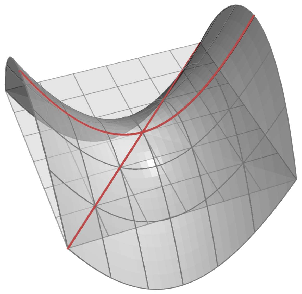
\includegraphics[hiresbb]{./figuras/paraboloide_hiperbolico+0_0.pdf}\hss}%
\includemedia[noplaybutton,3Dlights=Headlamp,3Dmenu,3Dtoolbar=false,label=paraboloide_hiperbolico,3Daac=20.925439825,3Dc2w=0.932039086 -0.362357754 0 -0.256225625 -0.659051158 0.707106781 -0.256225625 -0.659051158 -0.707106781 96.635465567 259.616728546 266.799613336,3Droo=384.517003998,3Dpsob=H,3Dbg=1 1 1,add3Djscript=asylabels.js]{\phantom{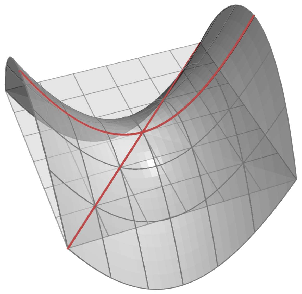
\includegraphics[hiresbb]{./figuras/paraboloide_hiperbolico+0_0.pdf}}}{./figuras/paraboloide_hiperbolico+0.prc}}%
